\documentclass{beamer}

\usetheme{Warsaw}
\usepackage{tikz}

\title[Solving the Graph Coloring Problem] % (optional, only for long titles)
{Problem Solving and Search in AI: Solving the Graph Coloring
Problem}
\author{Christian Wagner, Felix Winter}

\institute
{
  TU Wien  
}
\date[SS 2015] % (optional)
{Problem Solving and Search in AI: SS 2015}
\subject{Informatik}

\def\MLine#1{\par\hspace*{-\leftmargin}\parbox{\textwidth}{\[#1\]}}

\begin{document}
\section{Title}
  \frame{\titlepage}


\section{Introduction}

%% \begin{frame}
%%   \frametitle{The graphcoloring problem}


%%   Short explanation on the gcoloring problem
%%   \end{frame}

\section{Phase 1}
  \begin{frame}
    \frametitle{Overview of phase 1}

    \begin{enumerate}
      \item Algorithm description
      \item Used Methods
        \begin{itemize}
        \item{Inference techniques}
        \item{Variable- and Value-Selection heuristics}
        \item{Solving the optimization problem}
        \end{itemize}
        
      \item{Experiments}
        \begin{itemize}
        \item{Used Benchmarks}
        \item{Results}
        \item{Visualization of Solutions}
        \end{itemize}

    \end{enumerate}
  \end{frame}


  \begin{frame}
    \frametitle{Algorithm description}
    \begin{itemize}
    \item{Backtracking based algorithm}
    \item{Variables: Nodes of the graph}
    \item{Domains: Colors \{1 \dots k\}}
    \item{Constraints: $diff(n_1, n_2),  \forall (n_1, n_2) \in E$}
    \item{Constraint propagation and Variable/Value ordering used}
    \end{itemize}


  \end{frame}
\subsection{Used Methods}
\begin{frame}
    \frametitle{Inference techniques}
	Two different inference techniques:
	\begin{itemize}
	\item{Simple Forward Checking [FC]}	
		\begin{itemize}	
		\item{Establish arc-consistency between last assigned node and its neighbours}
		\end{itemize}
	\item{Maintain Arc Consistency [MAC]}
	\begin{itemize}	
		\item{Keep whole constraint graph consistent during the search}
		\end{itemize}
	\end{itemize}

  \end{frame}

\begin{frame}
    \frametitle{Variable- and Value-Selection heuristics}
	Variable selection heuristic:
	\begin{itemize}
	\item{Minimum Remaining Value [MRV]}
          \begin{itemize}
          \item{Variables with the least possible number of values preferred}
          \item{Ties are broken by Minimum Degree Heuristic}
          \end{itemize}
	\end{itemize}
	Value selection heuristic:
	\begin{itemize}
	\item{Least Constrained Value [LCV]}
          \begin{itemize}
          \item{Values which eliminate least colors in neighbour domains are preferred}
          \end{itemize}
          
	\end{itemize}
  \end{frame}

\begin{frame}
    \frametitle{Solving the optimization problem}
    \begin{itemize}
    \item{Only solves CSP}
	\item{Binary search by adapting k to find optimum}
	\end{itemize}
	\begin{block}{Binary search}
	$k = |V|/2, k_0 = 0, k_1 = |V|$\\
	$(k_0,k_1]$ is the range where the optimal solution lies\\
	If a k-colored solution exists\\
	\quad $k_1 = k$\\
	else\\
	\quad $k_0 = k$\\
	$k = k_0 + \frac{k_1 - k_0}{2}$\\
	stop if length of range is 1
	\end{block}
   \end{frame}
\subsection{Experiments}
\begin{frame}
    \frametitle{Used Benchmarks}
	
    \begin{itemize}
    \item{Three different variants of the algorithm}
        \begin{itemize}
        \item{FC + LCV}
        \item{MAC + LCV}
        \item{FC}
        \end{itemize}
    \item{MRV always used as it reduces running time significant}
        \begin{itemize}
        \item{e.g. on instance myciel4.col MRV faster by factor 10}
		\end{itemize}    
	\item{Tested on Quad-core 2.6 GHz, 8 GB RAM}
	\end{itemize}
	%server leistung, algo varianten etc.
  \end{frame}


\begin{frame}
    \frametitle{Results}

\begin{table}
  \tiny
        \begin{center}
          \begin{tabular}{r | r | r | r | r | r | r | r | r | r}
            \hline
             & \multicolumn{3}{c|}{Variant 1 FC+LCV} & \multicolumn{3}{c|}{Variant 2 MAC+LCV} & \multicolumn{3}{c}{Variant 3 FC} \\
            \hline
Instance & Time & k & optimal &  Time & k & optimal & Time & k & optimal \\
\hline \hline 
david.col & 10800s & 21 & no & 10800s & 21 & no & 10800s & 21 & no  \\
huck.col & 10800s & 19 & no & 10800s & 19 & no & 10800s & 19 & no \\
jean.col & 330.434s & 10 & yes & 1653.28s & 10 & yes & 288.373s & 10 & yes \\
queen5\_5.col & 0.017404s & 5 & yes & 0.058097s & 5 & yes & 0.009576s & 5 & yes  \\
queen6\_6.col & 13.645s & 7 & yes &  44.9005s & 7 & yes  & 11.7202s & 7 & yes \\
queen7\_7.col & 14.4932s & 7 & yes  & 62.4359s & 7 & yes & 12.5009s  & 7 & yes \\
queen8\_12.col & 10800s & 12 & yes &  10800s & 12 & yes & 10800s & 12 & yes  \\
queen8\_8.col & 10800s & 16  & no  & 10800s & 16 & no & 10800s & 16 & no \\
queen9\_9.col & 10800s & 10 & yes & 10800s & 10 & yes & 10800s & 10 & yes \\
myciel3.col &  0.005048s & 4 & yes & 0.00746s & 4 & yes  & 0.005062s & 4  & yes \\
myciel4.col & 0.445205s &  5& yes & 0.610285s & 5 & yes & 0.375327s & 5 & yes  \\
myciel5.col & 6973.74s & 6 & yes &10598.6s  & 6 & yes & 6187.41s & 6  & yes \\
myciel6.col & 10800s & 11 & no & 10800s & 11  & no & 10800s & 11 & no \\
\hline
\end{tabular}
        \caption{Table with results for the different variations and benchmark instances. FC: Simple Forward Checking, MAC: Maintaining Arc Consistency, LCV: Least Constrained Value heuristic }
        \label{myTable1}
        \end{center}
\end{table}

\end{frame}

\begin{frame}
  \frametitle{Visualization of Solutions}

  \begin{itemize}
    \item graphviz.org: open source graph library for drawing of graphs
  \end{itemize}

  \begin{figure}
    \footnotesize
   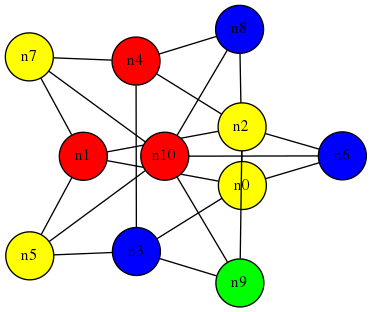
\includegraphics[width=0.475\textwidth]{myciel3.png}
   \hfill
   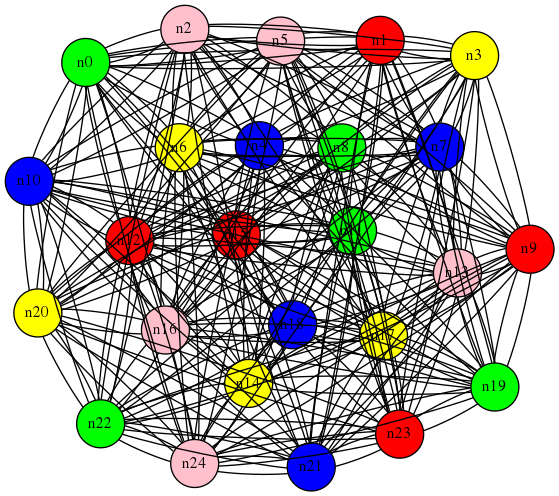
\includegraphics[width=0.475\textwidth]{queen5_5.png}
   \caption{The left side shows the optimal solution for myciel3.col and the right side for queen5\_5.png}
   \label{figure1}
\end{figure}

\end{frame}


\section{Phase 2}
  \begin{frame}
    \frametitle{Overview of phase 2}
    \begin{enumerate}

        \item Algorithm description
        \item Used Methods
          \begin{itemize}
            \item Problem formulation
            \item Neighbourhood operator
            \item Evaluation function
            \item Constructing an initial solution
          \end{itemize}
        \item Experiments
          \begin{itemize}
          \item Parameter configuration
          \item Best results
          \end{itemize}


    \end{enumerate}
  \end{frame}


\begin{frame}
    \frametitle{Algorithm description}

    \begin{itemize}
    \item Metaheuristic approach based on Tabu Search and Min-conflicts heuristic
    \item General Idea: Divide nodes into color classes and try to remove classes step by step
    \item Initial solution is constructed by algorithm from phase 1
    \end{itemize}

  \end{frame}

\subsection{Used Methods}
\begin{frame}
    \frametitle{Problem formulation}
\begin{itemize}
  \item Problem formulation is based on the paper Enrico Malaguti and Paolo Toth. Tabu search for the graph coloring problem.
    \item Nodes are divided into a number of color classes
    \end{itemize}
         \begin{block}{Definition}
           undirected graph $G = (V,E)$ \\
           solution $S$ is a partition of $V$ in $k+1$ color classes 
           $\lbrace V_1, V_2, V_3, ... V_{k+1} \rbrace$ \\
           all classes $V_i$ except the last one have to be a stable set
       \end{block}
    
  \end{frame}

\begin{frame}
    \frametitle{Neighbourhood operator}

    \begin{itemize}
    \item $V_{1..k}$ constitute a partial feasible $k$ coloring
    \item Making $V_{k+1}$ empty gives a complete feasible $k$ coloring
    \end{itemize}

       \begin{block}{Neighbourhood operator}
           choose an uncolored vertex $v \in V_{k+1}$ \\
           assign $v$ to different color class $h$\\
           move to class $k+1$ all vertices $v'$ from $h$ that are adjacent to $v$
       \end{block}

       \begin{itemize}
     \item the uncolored vertex $v$ is chosen randomly
     \item color class $h$ is chosen so that the number of generated conflicts is minimized
     \item From time to time $h$ is chosen randomly to introduce random noise (Random Walk)
     \item a tabu list stores the vertix pairs $(v,h)$ to cycles


       \end{itemize}

\end{frame}

\begin{frame}
    \frametitle{Evaluation function}

    \begin{itemize}
    \item simple variant could just count the number of nodes in class $V_{k+1}$
    \item Better: minimize the global degree of the uncolored vertices
    \end{itemize}

    \begin{block}{Evaluation function}
      $f(S) = \sum\limits_{v \in V_{k+1}} \delta(v)$\\
      where $\delta$ represents the degree of vertex $v$

      \end{block}

  \end{frame}

\begin{frame}
  \frametitle{Constructing an initial solution}
  \begin{itemize}
  \item initial solution has to be feasible for the algorithm to work
  \item we generate it by applying our algorithm from phase 1
  \item time for generating initial solution is 5\% of overall time limit
  \item first k has to be found anyway
\end{itemize}
  \end{frame}

\subsection{Experiments}

\begin{frame}
    \frametitle{Parameter configuration}
    \begin{itemize}
    \item 2 main parameters are used in our algorithm:
      \begin{itemize}
      \item probability for Random Walk
      \item length of tabu list relative to the number of nodes
      \end{itemize}

      
  \item We used irace 1.06.997 with its default configuration and all of the DJC*.col instances.
  \item time for one run was limited to 20 minutes
  \item because of the limited time we unfortunately had to cancel after 2 days and the first iteration.

  \item Elite candidates:
    \begin{itemize}
    \item p=5 tl=0.4729
    \item p=2 tl=0.4315

    \end{itemize}


    \end{itemize} 
  \end{frame}

\begin{frame}
    \frametitle{Best results}


  \begin{columns}
    \begin{column}{0.48\textwidth}
       \begin{table}
   \begin{tabular}{r | r | r |}
       
       Instance & k & optimal \\
       \hline 
       DSJC250.5.col & 33 & ? \\
       DSJC250.9.col & 79 & ? \\
       DSJC500.1.col & 14 & ? \\
       DSJC500.5.col & 60 & ? \\
       DSJC500.9.col & 152 & ? \\
       DSJR500.1.col & 12 & ? \\
       DSJR500.1c.col & 89 & ? \\
       DSJR500.5.col & 125 & ? \\
       latin\_square\_10.col & 124 & ? \\
       school1.col & 14 & ? \\
       school1\_nsh.col & 14 & ? \\
       \hline
   \end{tabular}
     \end{table}
    \end{column}
    \begin{column}{0.48\textwidth}
      \begin{table}
   \begin{tabular}{r | r | r }
       
       Instance & k & optimal \\
       \hline 
       queen10\_10.col & 12 & ? \\
       queen12\_12.col & 14 & ? \\
       queen14\_14.col & 16 & ? \\
       queen15\_15.col & 17 & ? \\
       queen16\_16.col & 18 & ? \\
       fpsol2.i.2.col & 30 & yes \\
       inithx.i.2.col & 31 & yes \\
       le450\_25b.col & 25 & yes \\
       miles1000.col & 42 &  yes \\
       mulsol.i.2.col & 31 & yes \\
       queen11\_11.col & 13 & no \\
       \hline
     \end{tabular}
      
     \end{table}

    \end{column}
\end{columns}
   

  \end{frame}



% slides for phase 2 insert here

  \section{Conclusion}
  \begin{frame}
    \frametitle{Conclusion and Discussion}


  \end{frame}


      %%   \begin{exampleblock}{Definition}
      %%   \emph{Constraint Optimization is the process of optimizing an objective function with respect to some variables in the presence of constraints}
      %% \end{exampleblock}

      %% \begin{itemize}
      %%   \item{Variety of practical problems can be modelled and solved}
      %%   \item{Very successful in the fields of scheduling, timetabling, routing, computational biology, ...}
      %% \end{itemize}


\begin{frame}
  \frametitle<presentation>{References}    
  \begin{thebibliography}{3}

    \beamertemplatebookbibitems
    \bibitem{ArtModern}
    Stuart Russel, Peter Norvig.
    \newblock {\em Artificial Intelligence. A Modern Approach}.
    \newblock Pearson Education, 2010.

    
  \beamertemplatearticlebibitems
  \bibitem{Tabu Search}
    Malaguti, Enrico and Toth, Paolo
    \newblock Tabu Search for the Graph Coloring Problem (extended)


  \bibitem{irace}
    L{\'o}pez-Ib{\'a}nez, Manuel and Dubois-Lacoste, J{\'e}r{\'e}mie and St{\"u}tzle, Thomas and Birattari, Mauro
    \newblock The irace package, iterated race for automatic algorithm configuration
    \newblock 2011


\bibitem{graphviz}
Ellson, John and Gansner, Emden and Koutsofios et al.
    \newblock Graphviz - open source graph drawing tools
    \newblock 2002
    
  \end{thebibliography}
\end{frame}

\begin{frame}
\frametitle{Questions}
\centerline{Any questions?}
\end{frame}


\end{document}
















